% 
\section{Kiến thức nền tảng}
\subsection{Bài toán tìm kiếm thông minh trong thương mại điện tử}
\subsubsection{Bài toán tìm kiếm sản phẩm trong E-commerce}

Trong các hệ thống thương mại điện tử hiện đại, tìm kiếm sản phẩm đóng vai trò quan trọng trong việc kết nối nhu cầu người dùng với dữ liệu sản phẩm. Khi số lượng sản phẩm ngày càng lớn, việc xây dựng cơ chế tìm kiếm hiệu quả trở thành yêu cầu cần thiết nhằm cải thiện trải nghiệm người dùng, rút ngắn thời gian tìm kiếm và tăng khả năng mua hàng.

Trên các nền tảng E-commerce lớn như Shopee và Lazada, bài toán tìm kiếm sản phẩm trở nên phức tạp do dữ liệu sản phẩm có quy mô rất lớn, đa dạng về ngành hàng, tên gọi, mô tả, hình ảnh, giá bán, thương hiệu và hành vi tương tác của người dùng. Một truy vấn đơn giản như ``áo khoác nam'', ``tai nghe bluetooth'' hoặc ``kem chống nắng cho da dầu'' có thể trả về hàng nghìn kết quả khác nhau. Do đó, hệ thống không chỉ cần tìm đúng sản phẩm có chứa từ khóa, mà còn phải xếp hạng các sản phẩm phù hợp nhất với ý định tìm kiếm của người dùng.

Các hệ thống truyền thống thường sử dụng keyword-based search bằng cách đối sánh trực tiếp từ khóa với tên sản phẩm hoặc mô tả. Tuy nhiên, phương pháp này gặp hạn chế với các truy vấn ngôn ngữ tự nhiên, truy vấn không đầy đủ, lỗi chính tả, từ đồng nghĩa hoặc truy vấn mang tính ngữ nghĩa. Ví dụ, người dùng có thể tìm kiếm ``giày đi học nữ'', trong khi sản phẩm lại được đặt tên là ``sneaker trắng nữ phong cách Hàn Quốc''. Nếu chỉ dựa trên đối sánh từ khóa, hệ thống có thể bỏ sót các sản phẩm phù hợp.

Bên cạnh đó, người dùng trên Shopee, Lazada và các nền tảng tương tự ngày càng có xu hướng tìm kiếm bằng nhiều dạng dữ liệu khác nhau như văn bản, hình ảnh hoặc kết hợp cả hai. Ví dụ, người dùng có thể chụp ảnh một chiếc túi hoặc đôi giày và yêu cầu hệ thống tìm các sản phẩm tương tự. Điều này dẫn đến sự phát triển của bài toán multimodal search, trong đó hệ thống cần xử lý đồng thời text, image và metadata sản phẩm để cải thiện chất lượng retrieval.

Sự phát triển của AI, đặc biệt là embedding model và deep learning, đã giúp các hệ thống AI Search có khả năng hiểu ngữ nghĩa truy vấn thay vì chỉ đối sánh từ khóa. Trong bối cảnh E-commerce, các kỹ thuật này có thể được sử dụng để biểu diễn truy vấn và sản phẩm dưới dạng vector embedding, từ đó tìm kiếm các sản phẩm có ý nghĩa gần nhau trong không gian ngữ nghĩa. Cách tiếp cận này phù hợp với các bài toán như semantic search, visual search, recommendation và conversational shopping assistant.

Đối với các nền tảng như Shopee và Lazada, một hệ thống tìm kiếm hiệu quả thường cần kết hợp nhiều yếu tố: mức độ liên quan giữa truy vấn và sản phẩm, độ phổ biến của sản phẩm, đánh giá từ người dùng, giá bán, tỷ lệ chuyển đổi, lịch sử hành vi người dùng và mức độ uy tín của nhà bán hàng. Vì vậy, bài toán tìm kiếm sản phẩm trong E-commerce không chỉ là bài toán retrieval đơn thuần, mà còn bao gồm cả ranking, personalization và optimization nhằm đưa ra kết quả phù hợp nhất với từng người dùng trong từng ngữ cảnh cụ thể.
\subsubsection{Hạn chế của Keyword-based Search}

Keyword-based search là phương pháp tìm kiếm truyền thống dựa trên việc đối sánh trực tiếp từ khóa truy vấn với nội dung dữ liệu. Các hệ thống này thường sử dụng kỹ thuật inverted index để tăng tốc độ truy xuất.

Mặc dù có ưu điểm về tốc độ xử lý và dễ triển khai, keyword search tồn tại nhiều hạn chế trong các bài toán semantic search hiện đại. Hệ thống không hiểu được ngữ nghĩa thực sự của câu truy vấn mà chỉ kiểm tra sự xuất hiện của từ khóa.

Ví dụ, khi người dùng tìm kiếm “giày chạy bộ nhẹ”, sản phẩm có mô tả “running sneakers with lightweight material” có thể không được trả về vì không chứa chính xác từ “giày” hoặc “nhẹ”. Điều này làm giảm độ chính xác retrieval.

Keyword search cũng gặp khó khăn trong các trường hợp:
\begin{itemize}
    \item Từ đồng nghĩa (shoe và sneaker)
    \item Viết sai chính tả
    \item Truy vấn dài bằng ngôn ngữ tự nhiên
    \item Tìm kiếm theo ngữ cảnh
    \item Truy vấn mô tả cảm xúc hoặc phong cách
\end{itemize}

Ngoài ra, keyword search không thể tự hiểu mối quan hệ ngữ nghĩa giữa các sản phẩm. Ví dụ, ``áo thể thao'' và ``sportswear'' có ý nghĩa tương tự, nhưng hệ thống tìm kiếm truyền thống khó nhận biết được nếu không được cấu hình trước bằng synonym dictionary, tức là một tập từ điển ánh xạ các từ hoặc cụm từ đồng nghĩa. Tuy nhiên, việc xây dựng synonym dictionary thường mang tính thủ công, tốn nhiều công sức và khó bao phủ hết các cách diễn đạt đa dạng của người dùng trong thực tế.
\subsubsection{Semantic Search}

Semantic Search là phương pháp tìm kiếm dựa trên ngữ nghĩa thay vì chỉ đối sánh từ khóa trực tiếp như keyword-based search truyền thống. Phương pháp này giúp hệ thống hiểu ý định người dùng và truy hồi các tài liệu hoặc sản phẩm có liên quan về mặt ngữ nghĩa dù không chứa chính xác từ khóa truy vấn.

Trong các hệ thống tìm kiếm hiện đại, semantic search thường được xây dựng dựa trên embedding model và vector retrieval. Hệ thống sẽ chuyển đổi truy vấn và tài liệu thành các vector embedding trong semantic space, nơi các dữ liệu có ý nghĩa tương đồng được biểu diễn gần nhau.

Ví dụ, các truy vấn như ``giày chạy bộ'', ``running shoes'' hoặc ``sports sneakers'' có thể được embedding thành các vector gần nhau bằng các model dù sử dụng các từ khác nhau. Điều này giúp cải thiện khả năng retrieval so với keyword matching truyền thống.

Semantic search thường bao gồm các bước như xử lý truy vấn, sinh embedding, truy xuất vector và xếp hạng kết quả theo độ tương đồng ngữ nghĩa.

\begin{figure}[H]
    \centering
    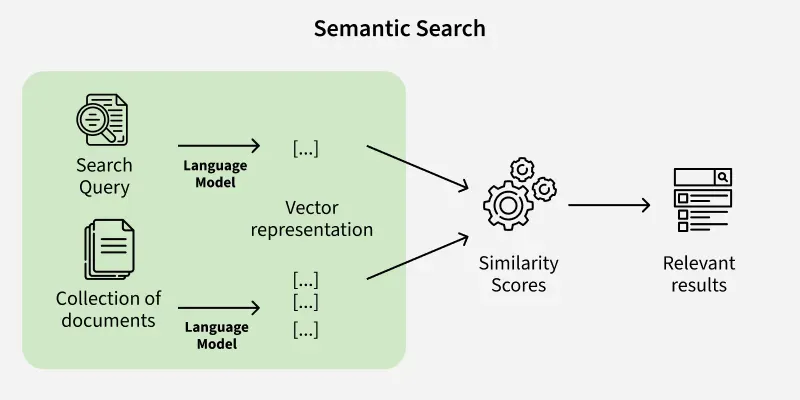
\includegraphics[width=0.75\textwidth]{Images/Kienthucnentang/Semantic-Search.png}
    \caption[Pipeline semantic search bao gồm các bước xử lý truy vấn, sinh embedding, truy xuất vector và xếp hạng kết quả dựa trên ngữ nghĩa]{Pipeline semantic search bao gồm các bước xử lý truy vấn, sinh embedding, truy xuất vector và xếp hạng kết quả dựa trên ngữ nghĩa \parencite{geeksforgeeks_semantic_search}}
    \label{fig:semantic_search_pipeline}
\end{figure}

Như minh họa trong \Cref{fig:semantic_search_pipeline}, semantic search sử dụng embedding vector để biểu diễn ngữ nghĩa của truy vấn và tài liệu trong không gian nhiều chiều, từ đó thực hiện semantic retrieval hiệu quả hơn keyword matching truyền thống.

Semantic search hiện là nền tảng quan trọng trong các hệ thống tìm kiếm thông minh, recommendation system và AI assistant hiện đại.
\subsubsection{Multimodal Search}

Multimodal Search là phương pháp tìm kiếm sử dụng nhiều loại dữ liệu như văn bản, hình ảnh và metadata để thực hiện truy hồi thông tin. Trong E-commerce, người dùng có thể tìm kiếm sản phẩm bằng hình ảnh hoặc kết hợp hình ảnh với mô tả văn bản như ``tìm áo giống hình này nhưng màu đen''.

Để giải quyết bài toán này, các hệ thống AI hiện đại thường sử dụng multimodal embedding nhằm ánh xạ dữ liệu từ nhiều modality vào cùng một semantic space. Các mô hình như CLIP sử dụng encoder riêng cho text và image, giúp các dữ liệu có ý nghĩa tương đồng được biểu diễn gần nhau trong vector space \cite{clip_paper}.

\begin{figure}[H]
    \centering
    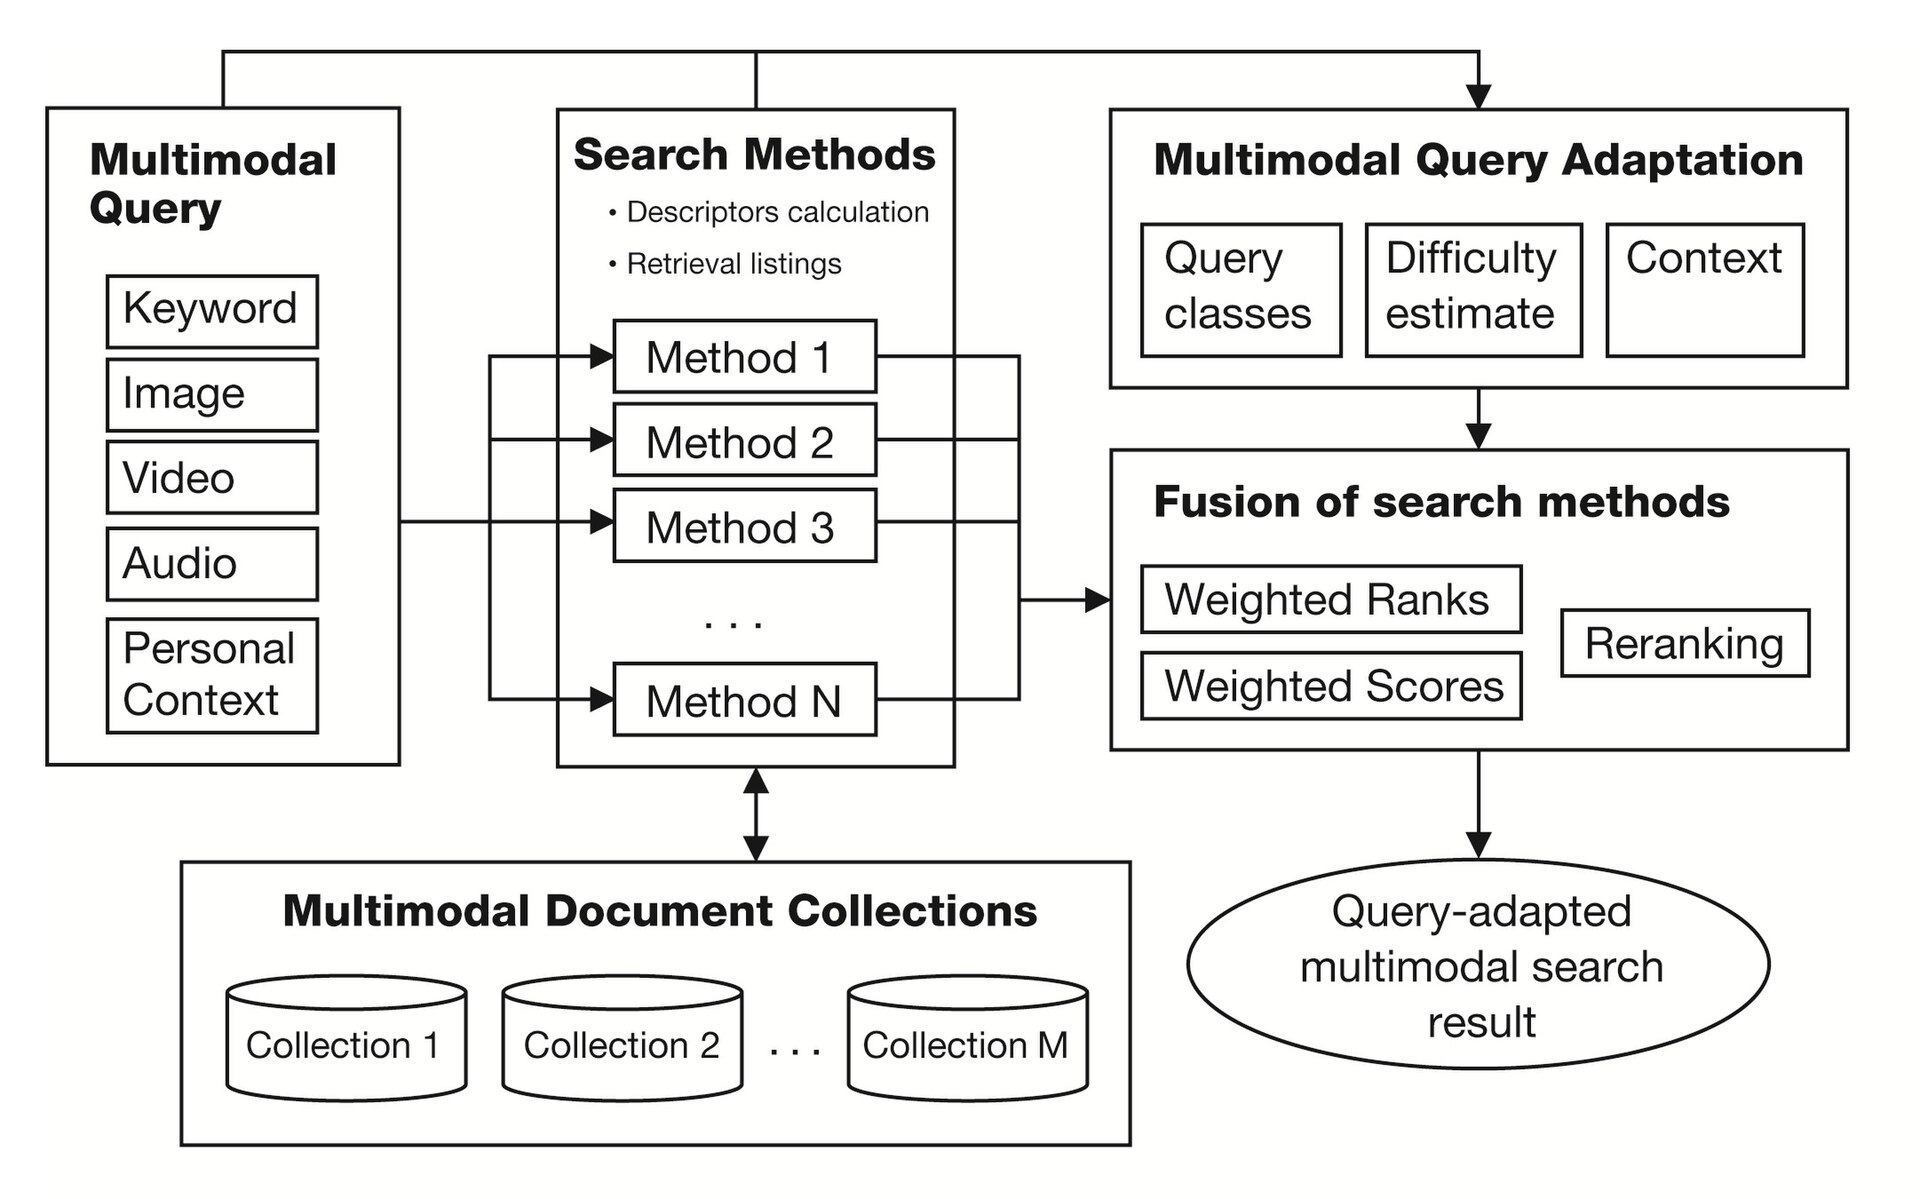
\includegraphics[width=0.7\textwidth]{Images/Kienthucnentang/Framework_of_Multimodal_Search.jpg}
    \caption[Framework của hệ thống multimodal search kết hợp truy vấn văn bản và hình ảnh nhằm cải thiện semantic retrieval trong E-commerce]{Framework của hệ thống multimodal search kết hợp truy vấn văn bản và hình ảnh nhằm cải thiện semantic retrieval trong E-commerce \parencite{ipullrank_mum_search}}
    \label{fig:framework_multimodal_search}
\end{figure}

Như trình bày trong \Cref{fig:framework_multimodal_search}, multimodal search kết hợp truy vấn văn bản và hình ảnh để cải thiện semantic retrieval thông qua embedding đa phương thức và vector retrieval.

Multimodal search hỗ trợ nhiều dạng truy hồi như text-to-image retrieval, image-to-image retrieval và hybrid retrieval, giúp cải thiện trải nghiệm tìm kiếm trong các hệ thống E-commerce hiện đại.
\subsubsection{Ứng dụng AI trong hệ thống tìm kiếm sản phẩm}

Trí tuệ nhân tạo đóng vai trò quan trọng trong các hệ thống tìm kiếm sản phẩm hiện đại. Khác với keyword-based search truyền thống, các hệ thống search dùng AI sử dụng embedding model và deep learning để khai thác ngữ nghĩa của truy vấn và dữ liệu sản phẩm.
Các ứng dụng AI phổ biến trong hệ thống E-commerce gồm:

\begin{itemize}
    \item \textbf{Semantic Search}: Hỗ trợ tìm kiếm sản phẩm dựa trên ý nghĩa của truy vấn thay vì chỉ đối sánh từ khóa.
    
    \item \textbf{Recommendation System}: Gợi ý sản phẩm phù hợp dựa trên hành vi người dùng, lịch sử tìm kiếm, lịch sử mua hàng hoặc sản phẩm tương tự.
    
    \item \textbf{Personalized Search}: Cá nhân hóa kết quả tìm kiếm theo sở thích, nhu cầu, vị trí, ngân sách hoặc lịch sử tương tác của từng người dùng.
    
    \item \textbf{Visual Search}: Cho phép người dùng tìm kiếm sản phẩm bằng hình ảnh, ví dụ tải lên ảnh một đôi giày hoặc chiếc túi để tìm sản phẩm tương tự.
    
    \item \textbf{Conversational AI Assistant}: Hỗ trợ người dùng tìm kiếm, so sánh và lựa chọn sản phẩm thông qua hội thoại tự nhiên.
\end{itemize}

AI giúp hệ thống hiểu ý định người dùng, phân tích ngữ cảnh truy vấn và cá nhân hóa kết quả tìm kiếm. Bên cạnh đó, sự phát triển của LLM và Conversational AI cho phép hỗ trợ hội thoại tự nhiên và tìm kiếm đa lượt hiệu quả hơn.

Việc kết hợp semantic search, recommendation system và multimodal retrieval hiện là xu hướng quan trọng trong các nền tảng E-commerce hiện đại.
\subsection{Hệ thống truy hồi thông tin}

% Hệ thống truy hồi thông tin (Information Retrieval -- IR) là lĩnh vực nghiên cứu tập trung vào việc tìm kiếm và truy xuất dữ liệu liên quan từ một tập dữ liệu lớn dựa trên truy vấn của người dùng \cite{manning_ir_book}. Trong lĩnh vực thương mại điện tử, hệ thống IR đóng vai trò quan trọng trong việc kết nối nhu cầu tìm kiếm của người dùng với cơ sở dữ liệu sản phẩm. Chất lượng của hệ thống truy hồi ảnh hưởng trực tiếp đến trải nghiệm người dùng, khả năng khám phá sản phẩm và hiệu quả recommendation.

% Khác với hệ quản trị cơ sở dữ liệu truyền thống chỉ truy xuất dữ liệu theo điều kiện chính xác, hệ thống IR tập trung vào việc đánh giá mức độ liên quan (relevance) giữa truy vấn và tài liệu. Điều này đặc biệt quan trọng trong các hệ thống tìm kiếm hiện đại khi người dùng thường sử dụng ngôn ngữ tự nhiên, truy vấn dài hoặc mô tả mang tính ngữ nghĩa thay vì các từ khóa cố định.

% Trong các hệ thống tìm kiếm hiện đại, Information Retrieval không chỉ bao gồm keyword matching truyền thống mà còn mở rộng sang semantic retrieval, vector retrieval, hybrid retrieval và reranking. Các hệ thống IR thường bao gồm các thành phần xử lý chính như:

% \begin{itemize}
%     \item Query processing
%     \item Candidate retrieval
%     \item Document ranking
%     \item Relevance refinement
%     \item Result presentation
% \end{itemize}

% Các phương pháp truy hồi truyền thống như TF-IDF hoặc BM25 chủ yếu dựa trên tần suất xuất hiện của từ khóa trong tài liệu \cite{bm25_paper}. Tuy nhiên, cùng với sự phát triển của deep learning và embedding model, nhiều hệ thống IR hiện đại đã chuyển sang sử dụng semantic embedding nhằm cải thiện khả năng hiểu ngữ nghĩa của truy vấn và dữ liệu.

% Ngoài độ chính xác retrieval, các hệ thống IR hiện đại còn phải đáp ứng nhiều yêu cầu khác như độ trễ thấp (low latency), khả năng mở rộng (scalability) và khả năng xử lý dữ liệu lớn trong thời gian thực. Đây là những yếu tố quan trọng trong các nền tảng thương mại điện tử và hệ thống tìm kiếm thông minh hiện nay.
% \subsubsection{Keyword-based Retrieval}

% Keyword-based Retrieval là phương pháp truy hồi thông tin truyền thống dựa trên việc đối sánh trực tiếp từ khóa truy vấn với nội dung dữ liệu \cite{manning_ir_book}. Đây là nền tảng của nhiều search engine cổ điển và vẫn được sử dụng rộng rãi trong các hệ thống tìm kiếm hiện nay nhờ tốc độ xử lý nhanh và chi phí tính toán thấp.

% Trong phương pháp này, hệ thống sẽ phân tích truy vấn của người dùng thành các token, sau đó tìm kiếm các tài liệu hoặc sản phẩm chứa các token tương ứng trong cơ sở dữ liệu. Để tăng tốc độ truy xuất, các hệ thống IR thường sử dụng cấu trúc dữ liệu inverted index \cite{lucene_docs}. Inverted index lưu ánh xạ giữa token và danh sách tài liệu chứa token đó, giúp giảm đáng kể thời gian tìm kiếm.

% Ví dụ, với truy vấn ``giày chạy bộ'', hệ thống sẽ tìm kiếm các tài liệu hoặc sản phẩm chứa các token như ``giày'', ``chạy'' và ``bộ'', sau đó tính toán mức độ liên quan dựa trên tần suất xuất hiện của từ khóa và các phương pháp xếp hạng như TF-IDF hoặc BM25 \cite{bm25_paper}.

% Ưu điểm của keyword-based retrieval bao gồm:

% \begin{itemize}
%     \item Tốc độ truy xuất nhanh
%     \item Dễ triển khai và tối ưu hóa
%     \item Chi phí tính toán thấp
%     \item Hoạt động hiệu quả với exact keyword matching
% \end{itemize}

% Tuy nhiên, keyword-based retrieval tồn tại nhiều hạn chế trong các hệ thống tìm kiếm hiện đại. Phương pháp này chủ yếu dựa trên token matching và không hiểu được ngữ nghĩa thực sự của truy vấn. Điều này làm giảm hiệu quả retrieval trong các trường hợp như:

% \begin{itemize}
%     \item Synonym và từ đồng nghĩa
%     \item Natural language query
%     \item Contextual meaning
%     \item Multilingual query
%     \item Conversational search
% \end{itemize}

% Ví dụ, các truy vấn như ``running shoes'', ``sports sneakers'' và ``giày chạy bộ'' có thể mang cùng ý nghĩa ngữ nghĩa nhưng lại được xem là các tập từ khóa khác nhau trong keyword retrieval truyền thống.

% Do những hạn chế về khả năng hiểu ngữ nghĩa, nhiều hệ thống tìm kiếm hiện đại thường kết hợp keyword-based retrieval với semantic retrieval nhằm tận dụng ưu điểm của cả hai phương pháp. Hướng tiếp cận này thường được gọi là hybrid search, trong đó keyword retrieval hỗ trợ xử lý exact matching còn semantic retrieval cải thiện khả năng hiểu ngữ cảnh và ý định truy vấn.
\subsubsection{BM25}

BM25 là một thuật toán xếp hạng được sử dụng phổ biến trong các hệ thống Information Retrieval truyền thống. Thuật toán này đánh giá mức độ liên quan giữa truy vấn và tài liệu dựa trên sự xuất hiện của từ khóa, đồng thời xét đến độ dài tài liệu để tránh việc các tài liệu dài luôn được ưu tiên hơn.

So với TF-IDF truyền thống, BM25 cải thiện khả năng xếp hạng nhờ cơ chế chuẩn hóa độ dài tài liệu, giảm ảnh hưởng của các từ xuất hiện quá nhiều và tối ưu điểm liên quan giữa truy vấn với tài liệu. Điểm BM25 thường được tính dựa trên ba yếu tố chính là tần suất xuất hiện của từ khóa trong tài liệu, mức độ hiếm của từ khóa trong toàn bộ tập tài liệu và độ dài của tài liệu.

Công thức tính điểm BM25 thường được biểu diễn như sau \cite{robertson2009probabilistic}:

\begin{equation}
\text{BM25}(q,d)=\sum_{t \in q} IDF(t)\cdot
\frac{f(t,d)\cdot (k_1+1)}
{f(t,d)+k_1\cdot
\left(1-b+b\cdot \frac{|d|}{avgdl}\right)}
\label{eq:bm25}
\end{equation}

Trong đó, $f(t,d)$ là số lần từ khóa $t$ xuất hiện trong tài liệu $d$, $|d|$ là độ dài tài liệu, $avgdl$ là độ dài tài liệu trung bình trong toàn bộ tập dữ liệu. Hai tham số $k_1$ và $b$ được dùng để điều chỉnh ảnh hưởng của tần suất từ khóa và mức độ chuẩn hóa theo độ dài tài liệu.

BM25 phù hợp với các truy vấn chứa từ khóa rõ ràng như tên sản phẩm, thương hiệu, mã sản phẩm hoặc thông số kỹ thuật. Tuy nhiên, do chủ yếu dựa trên token matching, BM25 còn hạn chế khi xử lý truy vấn ngôn ngữ tự nhiên, từ đồng nghĩa hoặc truy vấn phụ thuộc ngữ cảnh. Vì vậy, trong các hệ thống tìm kiếm hiện đại, BM25 thường được kết hợp với semantic retrieval để tạo thành hybrid retrieval.
\subsubsection{Semantic Retrieval}

Semantic Retrieval là phương pháp truy hồi thông tin dựa trên ngữ nghĩa thay vì chỉ đối sánh từ khóa trực tiếp như keyword-based retrieval truyền thống. Trong phương pháp này, truy vấn và tài liệu được biểu diễn dưới dạng vector embedding trong semantic space, nơi các dữ liệu có ý nghĩa tương đồng sẽ nằm gần nhau.

Semantic retrieval thường bao gồm các bước như query embedding, document embedding, vector similarity search và relevance ranking.
\begin{figure}[H]
    \centering
    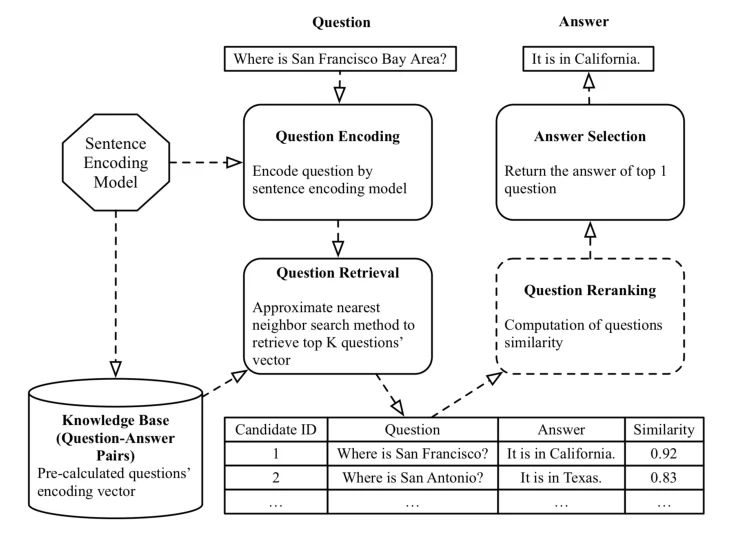
\includegraphics[width=0.65\textwidth]{Images/Kienthucnentang/semantic-retrieval.png}
    \caption[Workflow của semantic retrieval QA system bao gồm các bước embedding, semantic matching và retrieval]{Workflow của semantic retrieval QA system bao gồm các bước embedding, semantic matching và retrieval \parencite{semantic_retrieval_rg}}
    \label{fig:semantic_retrieval_workflow}
\end{figure}

Như minh họa trong \Cref{fig:semantic_retrieval_workflow}, semantic retrieval thực hiện truy xuất dựa trên độ tương đồng giữa các vector embedding thay vì chỉ dựa trên token matching truyền thống.
Ví dụ, với truy vấn ``áo khoác mùa đông'', hệ thống vẫn có thể truy hồi các sản phẩm như hoodie hoặc jacket dù không chứa chính xác từ khóa truy vấn.

Semantic retrieval giúp cải thiện khả năng hiểu ngữ nghĩa, hỗ trợ natural language query và tăng chất lượng retrieval trong các hệ thống tìm kiếm hiện đại. Tuy nhiên, việc xử lý vector embedding cũng làm tăng chi phí tính toán, do đó nhiều hệ thống hiện nay thường kết hợp semantic retrieval với keyword-based retrieval theo hướng hybrid retrieval.
% \subsubsection{Hybrid Search}

% Hybrid Search là phương pháp truy hồi thông tin kết hợp giữa keyword-based retrieval và semantic retrieval nhằm tận dụng ưu điểm của cả hai phương pháp \cite{hybrid_search_pinecone}.

% Trong khi keyword retrieval phù hợp với exact keyword hoặc brand name, semantic retrieval có khả năng xử lý ngữ nghĩa và natural language query tốt hơn. Hybrid search kết hợp sparse retrieval và dense retrieval để cải thiện chất lượng retrieval tổng thể.

% Hệ thống hybrid retrieval thường bao gồm BM25 retrieval, dense vector retrieval và fusion strategy như RRF.

% Ví dụ, với truy vấn ``nike running shoes under 2 million'', keyword retrieval hỗ trợ đối sánh thương hiệu ``Nike'', trong khi semantic retrieval giúp hiểu ngữ nghĩa của cụm ``running shoes''. Nhờ đó, hybrid search giúp cải thiện độ chính xác và hiệu quả retrieval trong các hệ thống tìm kiếm hiện đại.
% \subsubsection{Reranking}

% Reranking là giai đoạn sắp xếp lại các candidate document trong retrieval pipeline nhằm cải thiện mức độ liên quan giữa truy vấn và kết quả truy hồi \cite{reranking_sbert}.

% Thông thường, hệ thống retrieval gồm hai giai đoạn: first-stage retrieval để truy hồi top-k candidate nhanh chóng và second-stage reranking để đánh giá lại mức độ liên quan của từng kết quả.

% Khác với retrieval model chỉ dựa trên vector similarity, reranking thường sử dụng cross-encoder architecture để phân tích trực tiếp mối quan hệ giữa query và document, từ đó tính toán relevance score chính xác hơn.

% Ví dụ, với truy vấn ``giày chạy bộ cho người mới'', reranking model có thể ưu tiên các sản phẩm phù hợp với người mới thay vì các mẫu dành cho vận động viên chuyên nghiệp.

% Reranking giúp cải thiện retrieval precision và giảm irrelevant retrieval trong các hệ thống semantic search hiện đại. Tuy nhiên, do chi phí tính toán cao, phương pháp này thường chỉ áp dụng trên tập top-k candidate retrieval.
% \subsubsection{Đánh giá hệ thống truy hồi thông tin}

% Đánh giá hệ thống Information Retrieval (IR) là bước quan trọng nhằm đo lường hiệu quả retrieval của hệ thống tìm kiếm \cite{manning_ir_book}. Trong các hệ thống AI Search hiện đại, việc đánh giá không chỉ tập trung vào độ chính xác retrieval mà còn xem xét hiệu năng xử lý và khả năng đáp ứng yêu cầu thời gian thực.

% Các hệ thống IR thường được đánh giá dựa trên nhiều nhóm metric khác nhau, bao gồm retrieval effectiveness và system performance.

% \textbf{Precision}

% Precision đo tỷ lệ kết quả liên quan trong tập kết quả retrieval. Metric này phản ánh mức độ chính xác của hệ thống khi trả về các tài liệu hoặc sản phẩm phù hợp với truy vấn người dùng.

% Ví dụ, nếu hệ thống trả về top-10 kết quả và có 8 kết quả liên quan, precision sẽ bằng 0.8.

% \textbf{Recall}

% Recall đo khả năng truy hồi đầy đủ các tài liệu liên quan trong toàn bộ corpus.

% Metric này đặc biệt quan trọng trong các hệ thống semantic retrieval vì mục tiêu không chỉ là trả về kết quả chính xác mà còn hạn chế bỏ sót các tài liệu liên quan.

% \textbf{MRR (Mean Reciprocal Rank)}

% MRR được sử dụng để đánh giá vị trí xuất hiện của kết quả đúng đầu tiên trong danh sách retrieval.

% MRR có ý nghĩa quan trọng trong các hệ thống tìm kiếm sản phẩm hoặc question answering, nơi người dùng thường ưu tiên các kết quả đầu tiên.

% \textbf{nDCG (Normalized Discounted Cumulative Gain)}

% nDCG là metric đánh giá chất lượng ranking dựa trên mức độ liên quan và vị trí của kết quả retrieval.

% Metric này cho phép đánh giá chất lượng xếp hạng trong các hệ thống retrieval có nhiều mức relevance khác nhau.

% Ngoài các retrieval metric, hệ thống IR hiện đại còn được đánh giá dựa trên các yếu tố hiệu năng như:

% \begin{itemize}
%     \item Latency
%     \item Throughput
%     \item Scalability
%     \item Resource utilization
% \end{itemize}

% Trong các hệ thống AI Shopping Assistant, retrieval quality ảnh hưởng trực tiếp đến chất lượng tìm kiếm, recommendation và phản hồi của hệ thống RAG. Vì vậy, việc lựa chọn metric đánh giá phù hợp đóng vai trò quan trọng trong quá trình tối ưu hệ thống retrieval.

% Nhiều benchmark Information Retrieval hiện đại như BEIR được sử dụng để đánh giá retrieval model trên nhiều domain và retrieval task khác nhau \cite{beir_benchmark}.
\subsection{Vector Embedding và Semantic Representation}
\subsubsection{Khái niệm Vector Embedding}

Trong các hệ thống AI Search hiện đại, dữ liệu thường được chuyển đổi thành các vector số học nhằm hỗ trợ máy tính biểu diễn và xử lý ngữ nghĩa của dữ liệu \cite{bert_paper}. Vector embedding là phương pháp ánh xạ dữ liệu như văn bản hoặc hình ảnh thành các vector trong không gian nhiều chiều, trong đó khoảng cách giữa các vector phản ánh mức độ tương đồng ngữ nghĩa giữa các đối tượng dữ liệu.

Khác với các phương pháp biểu diễn truyền thống, embedding cho phép mô hình học được mối quan hệ ngữ nghĩa giữa dữ liệu. Nhờ đó, các cụm từ như ``giày chạy bộ'', ``running shoes'' hay ``sports sneakers'' có thể được biểu diễn bằng các vector gần nhau dù sử dụng từ khác nhau.

Embedding đóng vai trò quan trọng trong semantic retrieval và multimodal search. Sau khi dữ liệu được embedding hóa, hệ thống có thể thực hiện similarity search hoặc vector retrieval để tìm các đối tượng có mức độ tương đồng cao trong semantic space.

Hiện nay, vector embedding được ứng dụng rộng rãi trong semantic search, recommendation system, chatbot và RAG.
\subsubsection{Semantic Space}

Semantic space là không gian biểu diễn vector trong đó khoảng cách giữa các vector phản ánh mức độ tương đồng ngữ nghĩa giữa các dữ liệu \cite{pinecone_embedding}. Sau khi dữ liệu được embedding hóa, các vector sẽ được ánh xạ vào semantic space để phục vụ các bài toán semantic retrieval và similarity search.

Ý tưởng cốt lõi của semantic space là các dữ liệu có nội dung tương tự sẽ nằm gần nhau trong không gian vector dù sử dụng cách biểu diễn khác nhau. Ví dụ, các cụm từ như ``laptop gaming'', ``gaming notebook'' và ``máy tính chơi game'' có thể được biểu diễn bằng các vector gần nhau do mang ý nghĩa tương đồng.

Để đo mức độ tương đồng giữa các vector trong semantic space, các hệ thống retrieval thường sử dụng các phép đo như:

\begin{itemize}
    \item Cosine Similarity
    \item Euclidean Distance
    \item Dot Product
\end{itemize}

Trong đó, Cosine Similarity là phương pháp phổ biến nhất trong semantic retrieval do tập trung đo sự tương đồng về hướng của vector thay vì độ lớn tuyệt đối.

Một đặc điểm quan trọng của semantic space là hiện tượng semantic clustering, trong đó các vector có cùng chủ đề hoặc đặc trưng dữ liệu thường hình thành các cụm trong không gian vector. Điều này hỗ trợ hiệu quả cho các hệ thống semantic search và recommendation system.

Tuy nhiên, khi số lượng vector tăng lên rất lớn, việc tìm kiếm nearest neighbors trong semantic space trở nên tốn kém về mặt tính toán. Vì vậy, các hệ thống hiện đại thường sử dụng vector database và ANN indexing nhằm tối ưu tốc độ retrieval.
\subsubsection{Text Embedding}

Text Embedding là kỹ thuật chuyển đổi văn bản thành vector số thực nhằm biểu diễn ngữ nghĩa của câu, đoạn văn hoặc tài liệu trong không gian vector. Đây là nền tảng quan trọng của nhiều hệ thống NLP hiện đại như semantic search, recommendation system, chatbot và RAG.

Khác với các phương pháp truyền thống như bag-of-words hoặc TF-IDF, text embedding cho phép mô hình học được semantic representation của ngôn ngữ tự nhiên. Nhờ đó, các câu hoặc cụm từ có ý nghĩa tương đồng sẽ được biểu diễn gần nhau trong semantic space.

Trong hệ thống AI Shopping Assistant, text embedding được sử dụng để biểu diễn product title, product description, user query và conversational context.

Ví dụ, các truy vấn như ``running shoes'', ``sports sneakers'' và ``giày chạy bộ'' có thể được ánh xạ gần nhau trong semantic space.

Hiện nay, nhiều hệ thống semantic search sử dụng transformer-based embedding model như BERT hoặc Sentence-BERT nhằm cải thiện chất lượng semantic retrieval.
\subsubsection{Image Embedding}

Image Embedding là kỹ thuật chuyển đổi hình ảnh thành vector số thực nhằm biểu diễn đặc trưng trực quan và ngữ nghĩa của ảnh trong không gian vector. Đây là nền tảng quan trọng trong các hệ thống computer vision hiện đại như image retrieval, visual search và multimodal AI.

Khác với các phương pháp xử lý ảnh truyền thống, image embedding sử dụng deep learning để tự động học đặc trưng của hình ảnh. Các hình ảnh có nội dung tương tự sẽ được biểu diễn bằng các vector nằm gần nhau trong semantic space.

Trong hệ thống AI Shopping Assistant, image embedding được sử dụng để biểu diễn product image, user uploaded image và visual feature representation.

Ví dụ, khi người dùng tải lên hình ảnh của một đôi giày thể thao, hệ thống sẽ chuyển đổi hình ảnh thành vector embedding và thực hiện similarity search để tìm các sản phẩm tương tự.

Hiện nay, nhiều hệ thống AI hiện đại sử dụng các mô hình như CLIP, ViT hoặc CNN để xây dựng image embedding phục vụ visual search và multimodal retrieval.
\subsubsection{Multimodal Embedding}

Multimodal Embedding là kỹ thuật biểu diễn nhiều loại dữ liệu như văn bản và hình ảnh trong cùng một semantic space. Đây là nền tảng quan trọng của các hệ thống multimodal AI và cross-modal retrieval hiện đại.

Trong multimodal embedding, hệ thống sử dụng các encoder riêng cho text và image nhưng được huấn luyện để tạo ra embedding trong cùng không gian vector. Nhờ đó, dữ liệu có cùng ý nghĩa ngữ nghĩa sẽ được biểu diễn gần nhau dù thuộc các modality khác nhau.

Ví dụ, truy vấn ``áo hoodie màu đen'' và hình ảnh của một áo hoodie đen có thể được ánh xạ thành các vector gần nhau trong semantic space.

Multimodal embedding hỗ trợ nhiều bài toán như text-to-image retrieval, image-to-text retrieval và hybrid search. Trong E-commerce, kỹ thuật này giúp người dùng tìm kiếm sản phẩm linh hoạt hơn bằng cách kết hợp văn bản và hình ảnh.

Hiện nay, nhiều mô hình như CLIP, SigLIP hoặc ALIGN được sử dụng để xây dựng multimodal embedding phục vụ semantic retrieval và multimodal search.
% \subsubsection{Tiêu chí lựa chọn mô hình Text Embedding}
% Việc lựa chọn mô hình text embedding là bước quan trọng trong quá trình xây dựng hệ thống AI Search và semantic retrieval. Một mô hình embedding phù hợp không chỉ ảnh hưởng đến độ chính xác retrieval mà còn tác động trực tiếp đến latency, scalability và chi phí triển khai của hệ thống.

% Tiêu chí đầu tiên cần xem xét là semantic performance. Đây là yếu tố quan trọng nhất trong các hệ thống AI Search hiện đại vì mục tiêu chính của embedding là biểu diễn ngữ nghĩa của dữ liệu. Mô hình cần có khả năng đưa các câu hoặc truy vấn có ý nghĩa tương tự đến gần nhau trong semantic space. Trong bài toán thương mại điện tử, điều này đặc biệt quan trọng vì người dùng thường sử dụng truy vấn ngôn ngữ tự nhiên thay vì exact keyword.

% Tiêu chí thứ hai là retrieval quality. Một mô hình embedding tốt cần tối ưu cho semantic retrieval thay vì chỉ phục vụ NLP thông thường. Các mô hình được huấn luyện bằng contrastive learning như BGE hoặc E5 thường cho hiệu quả retrieval cao hơn trong các bài toán vector search và RAG.

% Embedding dimension cũng là yếu tố quan trọng cần cân nhắc. Vector dimension càng lớn thì khả năng biểu diễn semantic càng mạnh nhưng đồng thời cũng làm tăng:
% Các tiêu chí quan trọng:
% \begin{itemize}
%     \item Bộ nhớ lưu trữ vector
%     \item Chi phí ANN indexing
%     \item Latency retrieval
%     \item GPU memory usage
% \end{itemize}

% Ví dụ, embedding 3072 chiều sẽ yêu cầu nhiều tài nguyên hơn embedding 384 chiều khi lưu trữ hàng triệu sản phẩm trong vector database. Vì vậy, hệ thống thực tế thường cần cân bằng giữa semantic quality và scalability

% Latency và inference speed cũng là tiêu chí quan trọng trong hệ thống E-commerce Search thời gian thực. Người dùng thường kỳ vọng kết quả tìm kiếm được trả về trong vài trăm milliseconds. Do đó, embedding model cần đủ nhẹ để inference nhanh nhưng vẫn đảm bảo semantic quality. Các mô hình small hoặc base thường phù hợp hơn large model trong môi trường production do tối ưu tốt hơn về tốc độ và chi phí vận hành.

% Khả năng hỗ trợ multilingual retrieval là tiêu chí cần thiết trong các hệ thống thương mại điện tử đa ngôn ngữ. Người dùng có thể tìm kiếm bằng tiếng Anh, tiếng Việt hoặc kết hợp nhiều ngôn ngữ khác nhau. Các mô hình như multilingual-E5 hoặc BGE-M3 thường có ưu thế trong các bài toán multilingual semantic search.

% Ngoài ra, khả năng self-hosting và triển khai nội bộ cũng là yếu tố quan trọng trong nhiều hệ thống doanh nghiệp. Open-source embedding model như BGE hoặc E5 cho phép triển khai trực tiếp trên server nội bộ, giúp:

% \begin{itemize}
%     \item Giảm chi phí API
%     \item Bảo vệ dữ liệu người dùng
%     \item Tùy chỉnh theo domain riêng
%     \item Chủ động tối ưu pipeline retrieval
% \end{itemize}

% Trong đồ án AI Shopping Assistant, mô hình BGE được lựa chọn do đáp ứng tốt các tiêu chí:
% \begin{itemize}
%     \item Semantic retrieval mạnh
%     \item Tối ưu cho dense retrieval
%     \item Hỗ trợ multilingual
%     \item Hoạt động tốt với vector database
%     \item Phù hợp hybrid search và RAG pipeline
%     \item Có phiên bản lightweight cho inference nhanh
% \end{itemize}
% Ngoài ra, BGE có hệ sinh thái hỗ trợ tốt cho semantic search và retrieval engineering, giúp dễ dàng tích hợp với Qdrant, LangChain và các vector database hiện đại
% \subsubsection{Tiêu chí lựa chọn mô hình Image Embedding}

% Khi lựa chọn mô hình embedding cho hệ thống AI search hoặc CBIR, cần cân nhắc các yếu tố sau:

% \begin{itemize}
%     \item \textbf{Độ chính xác (Accuracy)}
%     \item \textbf{Tốc độ suy luận (Inference speed)}
%     \item \textbf{Khả năng mở rộng (Scalability)}
%     \item \textbf{Chi phí huấn luyện}
%     \item \textbf{Tính sẵn có của pretrained model}
% \end{itemize}

% Trong thực tế, các hệ thống thương mại thường sử dụng:
% \begin{itemize}
%     \item CNN (ResNet, EfficientNet) cho baseline
%     \item Vision Transformer hoặc CLIP cho semantic search nâng cao
% \end{itemize}
\subsection{Multimodal Search trong E-commerce}

\subsubsection{Text-Image Retrieval}

Text-Image Retrieval là bài toán truy xuất dữ liệu giữa văn bản và hình ảnh, trong đó hệ thống thực hiện tìm kiếm hình ảnh từ văn bản hoặc tìm kiếm văn bản từ hình ảnh \parencite{faghri2018vsepp}.

Mục tiêu của phương pháp này là học mối quan hệ ngữ nghĩa giữa text và image bằng cách ánh xạ chúng vào cùng một semantic embedding space. Trong không gian này, các cặp dữ liệu có liên quan sẽ có khoảng cách vector gần nhau hơn.

Trong hệ thống retrieval hiện đại, văn bản thường được xử lý bởi text encoder và hình ảnh được xử lý bởi image encoder nhằm trích xuất semantic feature cho từng modality.

Các thành phần chính của text-image retrieval gồm:
\begin{itemize}
    \item Text Representation
    \item Image Representation
    \item Shared Embedding Space
    \item Similarity Measurement
\end{itemize}

\begin{figure}[H]
    \centering
    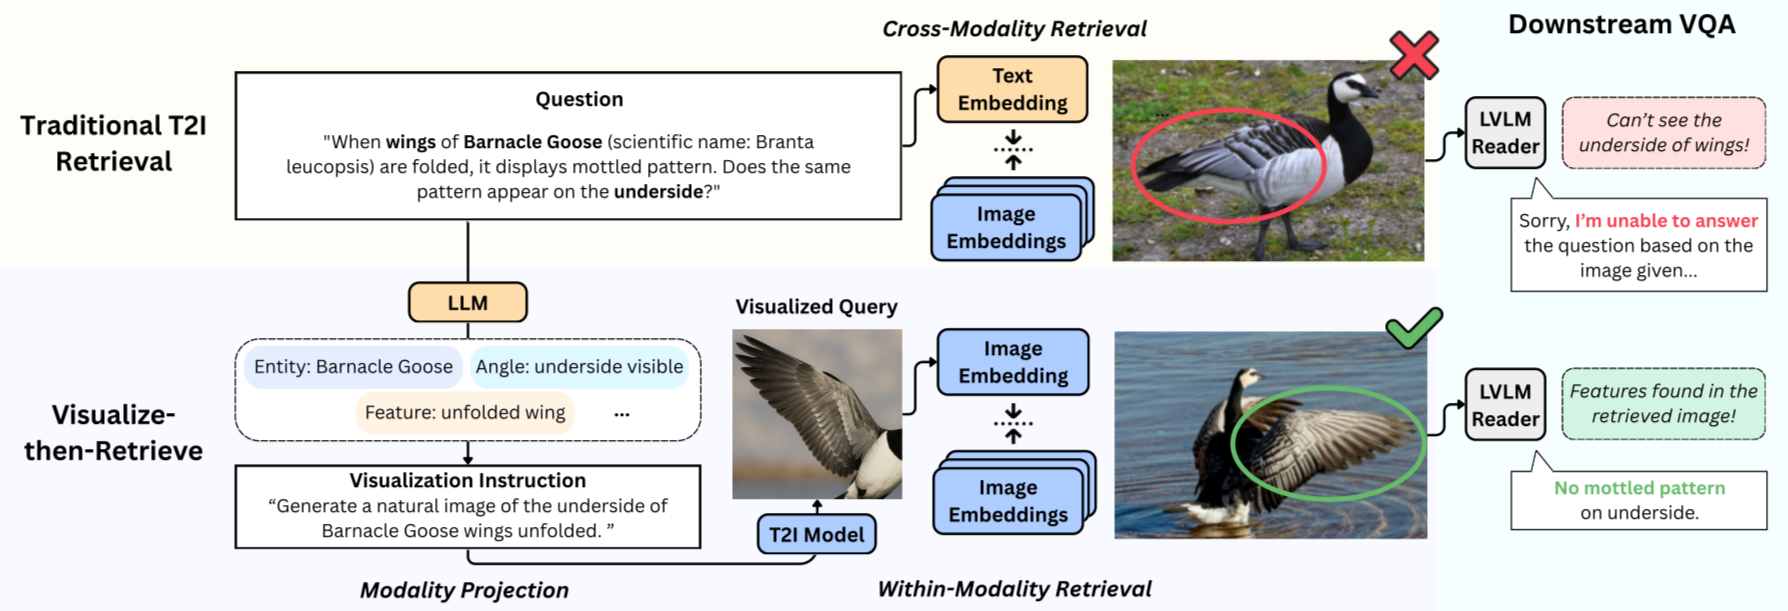
\includegraphics[width=0.75\linewidth]{Images/Kienthucnentang/text-image-retrieval.png}
    \caption[Bài toán Text-Image Retrieval với quá trình ánh xạ văn bản và hình ảnh vào cùng không gian ngữ nghĩa để thực hiện truy xuất liên modality]{Bài toán Text-Image Retrieval với quá trình ánh xạ văn bản và hình ảnh vào cùng không gian ngữ nghĩa để thực hiện truy xuất liên modality \cite{moonlight2024visualizedretrieval}}
    \label{fig:text-image-retrieval}
\end{figure}

Như minh họa ở \Cref{fig:text-image-retrieval}, text-image retrieval hỗ trợ liên kết dữ liệu văn bản và hình ảnh nhằm phục vụ các hệ thống multimodal search và E-commerce retrieval hiện đại.
\subsubsection{Computer Vision và Object Detection trong E-commerce}

Computer Vision là lĩnh vực cho phép máy tính phân tích và hiểu thông tin từ hình ảnh hoặc video. Trong thương mại điện tử, Computer Vision được ứng dụng nhằm hỗ trợ phân tích sản phẩm, visual search, visual recommendation và hiểu nội dung hình ảnh sản phẩm.

Dữ liệu hình ảnh đóng vai trò quan trọng trong E-commerce vì người dùng thường đưa ra quyết định mua sắm dựa trên thông tin trực quan. Các kỹ thuật Computer Vision giúp hệ thống khai thác các đặc trưng thị giác như màu sắc, hình dạng, kết cấu, kiểu dáng hoặc phong cách của sản phẩm từ dữ liệu hình ảnh. Những đặc trưng này có thể được sử dụng để tìm kiếm sản phẩm tương tự, phân loại sản phẩm hoặc hỗ trợ hệ thống gợi ý sản phẩm theo ngữ cảnh thị giác.

Trong các hệ thống E-commerce hiện đại, Computer Vision thường được sử dụng cho các bài toán:
\begin{itemize}
    \item Nhận dạng và phân loại sản phẩm
    \item Tìm kiếm sản phẩm bằng hình ảnh
    \item Phân tích thuộc tính thị giác của sản phẩm
    \item Phát hiện đối tượng trong ảnh sản phẩm
    \item Visual recommendation và visual retrieval
\end{itemize}
\begin{figure}[H]
    \centering
    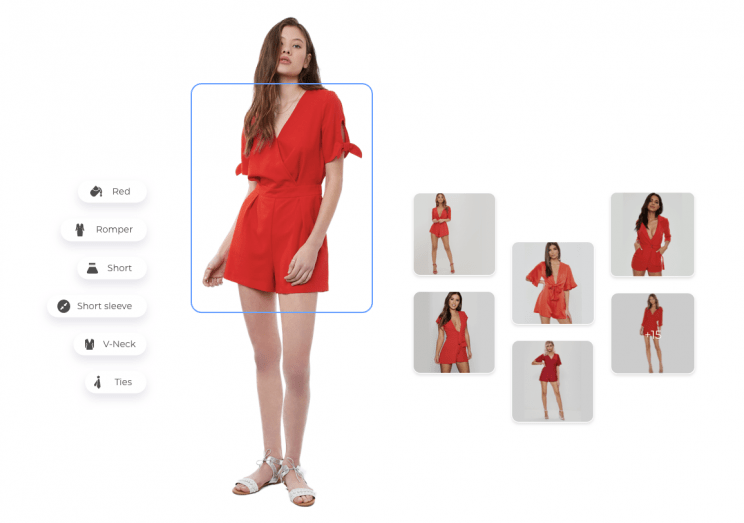
\includegraphics[width=0.7\textwidth]{Images/Kienthucnentang/visual-search-ecommerce.png}
    \caption[Ứng dụng Computer Vision trong tìm kiếm sản phẩm bằng hình ảnh trong E-commerce]{Ứng dụng Computer Vision trong tìm kiếm sản phẩm bằng hình ảnh trong E-commerce \parencite{cleed2024visualsearch}}
    \label{fig:visual-search-ecommerce}
\end{figure}
Một thành phần quan trọng của Computer Vision là visual feature representation, trong đó hình ảnh được chuyển đổi thành vector đặc trưng để biểu diễn nội dung thị giác trong không gian nhiều chiều. Các vector này hỗ trợ việc đo độ tương đồng giữa các hình ảnh và phục vụ semantic retrieval trong hệ thống AI Shopping Assistant.

Trong phạm vi Computer Vision, Object Detection là bài toán nhằm xác định vị trí và phân loại các đối tượng xuất hiện trong hình ảnh hoặc video \parencite{redmon2016yolo}. Khác với image classification chỉ dự đoán nhãn cho toàn bộ ảnh, Object Detection yêu cầu hệ thống vừa nhận diện loại đối tượng vừa xác định vị trí của chúng thông qua bounding box.

Trong Object Detection, mô hình thường thực hiện hai nhiệm vụ chính:
\begin{itemize}
    \item \textbf{Localization}: Xác định vị trí đối tượng trong ảnh.
    \item \textbf{Classification}: Phân loại đối tượng được phát hiện.
\end{itemize}

Kết quả của Object Detection thường bao gồm nhãn đối tượng, tọa độ bounding box và confidence score. Các thành phần quan trọng của Object Detection gồm feature extraction, bounding box regression và object classification. Một số mô hình còn sử dụng region proposal hoặc dense prediction để xác định các vùng có khả năng chứa đối tượng.

Các mô hình Object Detection hiện đại thường được chia thành hai nhóm chính:
\begin{itemize}
    \item \textbf{Two-stage Detector}: thực hiện đề xuất vùng trước, sau đó phân loại và tinh chỉnh bounding box, ví dụ như R-CNN và Faster R-CNN.
    \item \textbf{One-stage Detector}: dự đoán trực tiếp bounding box và nhãn đối tượng trong một lần xử lý, ví dụ như YOLO và SSD.
\end{itemize}

Trong đó, YOLO là một trong những mô hình Object Detection phổ biến nhờ khả năng xử lý thời gian thực và hiệu quả cao trong nhiều bài toán Computer Vision. Đối với E-commerce, Object Detection có thể được sử dụng để phát hiện sản phẩm trong ảnh, nhận diện nhiều sản phẩm xuất hiện cùng lúc, trích xuất vùng ảnh chứa sản phẩm chính và hỗ trợ tìm kiếm sản phẩm bằng hình ảnh. Ví dụ, khi người dùng tải lên một bức ảnh có chứa áo, giày hoặc túi xách, hệ thống có thể phát hiện từng đối tượng trong ảnh, cắt vùng liên quan và sử dụng đặc trưng thị giác của đối tượng đó để truy xuất các sản phẩm tương tự trong cơ sở dữ liệu.

Như vậy, Computer Vision cung cấp nền tảng tổng quát để hệ thống hiểu dữ liệu hình ảnh, trong khi Object Detection đóng vai trò là một kỹ thuật cụ thể giúp nhận diện và định vị sản phẩm trong ảnh. Sự kết hợp này giúp cải thiện khả năng visual search, product retrieval và trải nghiệm mua sắm trực quan trong các hệ thống E-commerce hiện đại.
\subsection{Vector Database và ANN Search}

\subsubsection{Khái niệm Vector Database}

Vector Database là loại cơ sở dữ liệu dùng để quản lý các vector embedding được tạo ra từ dữ liệu như văn bản, hình ảnh hoặc sản phẩm \parencite{wang2021milvus}. Thay vì chỉ tìm kiếm theo điều kiện khớp chính xác như cơ sở dữ liệu truyền thống, Vector Database cho phép truy xuất các đối tượng có mức độ tương đồng cao trong không gian vector. Nhờ đó, hệ thống có thể tìm ra những kết quả gần nghĩa hoặc gần đặc trưng với truy vấn đầu vào.

Trong các hệ thống AI hiện đại, dữ liệu như văn bản hoặc hình ảnh thường được chuyển đổi thành embedding vector nhằm biểu diễn semantic feature của dữ liệu. Các vector này cho phép hệ thống thực hiện semantic search và retrieval hiệu quả hơn keyword matching truyền thống.

Vector database đóng vai trò quan trọng trong semantic search, recommendation system, multimodal retrieval và RAG. Thay vì tìm kiếm theo từ khóa chính xác, hệ thống sẽ truy xuất các vector có khoảng cách gần nhất với vector truy vấn trong embedding space.

Các thành phần chính của vector database gồm:
\begin{itemize}
    \item Vector Embedding
    \item Vector Index
    \item Similarity Search
    \item High-dimensional Space
\end{itemize}

Trong không gian vector, các dữ liệu có ý nghĩa tương đồng thường được biểu diễn gần nhau hơn, giúp hệ thống hỗ trợ semantic retrieval hiệu quả.
\subsubsection{Độ tương đồng vector và Vector Similarity}

Sau khi dữ liệu được biểu diễn dưới dạng vector embedding, hệ thống AI Search cần một phương pháp để so sánh mức độ gần nhau giữa các vector. Việc đo độ tương đồng này giúp hệ thống xác định những sản phẩm, tài liệu hoặc truy vấn có ý nghĩa gần nhau, từ đó hỗ trợ các tác vụ như semantic retrieval và recommendation system.

Trong hệ thống tìm kiếm sản phẩm, truy vấn của người dùng sẽ được embedding hóa thành vector và so sánh với các vector sản phẩm trong vector database. Các vector có khoảng cách gần nhau hơn sẽ được xem là có mức độ liên quan cao hơn.

Khác với keyword matching truyền thống, vector similarity cho phép hệ thống hiểu semantic meaning thay vì exact keyword. Ví dụ, các cụm từ như ``running shoes'', ``sports sneakers'' và ``giày chạy bộ'' có thể được đánh giá tương đồng dù sử dụng từ khác nhau.

Một số phép đo vector similarity phổ biến gồm:
\begin{itemize}
    \item \textbf{Cosine Similarity}
    \item \textbf{Euclidean Distance}
    \item \textbf{Dot Product}
\end{itemize}

Trong đó, Cosine Similarity là phương pháp được sử dụng phổ biến trong semantic retrieval do khả năng đánh giá mức độ tương đồng ngữ nghĩa giữa các vector embedding.

\begin{figure}[H]
    \centering
    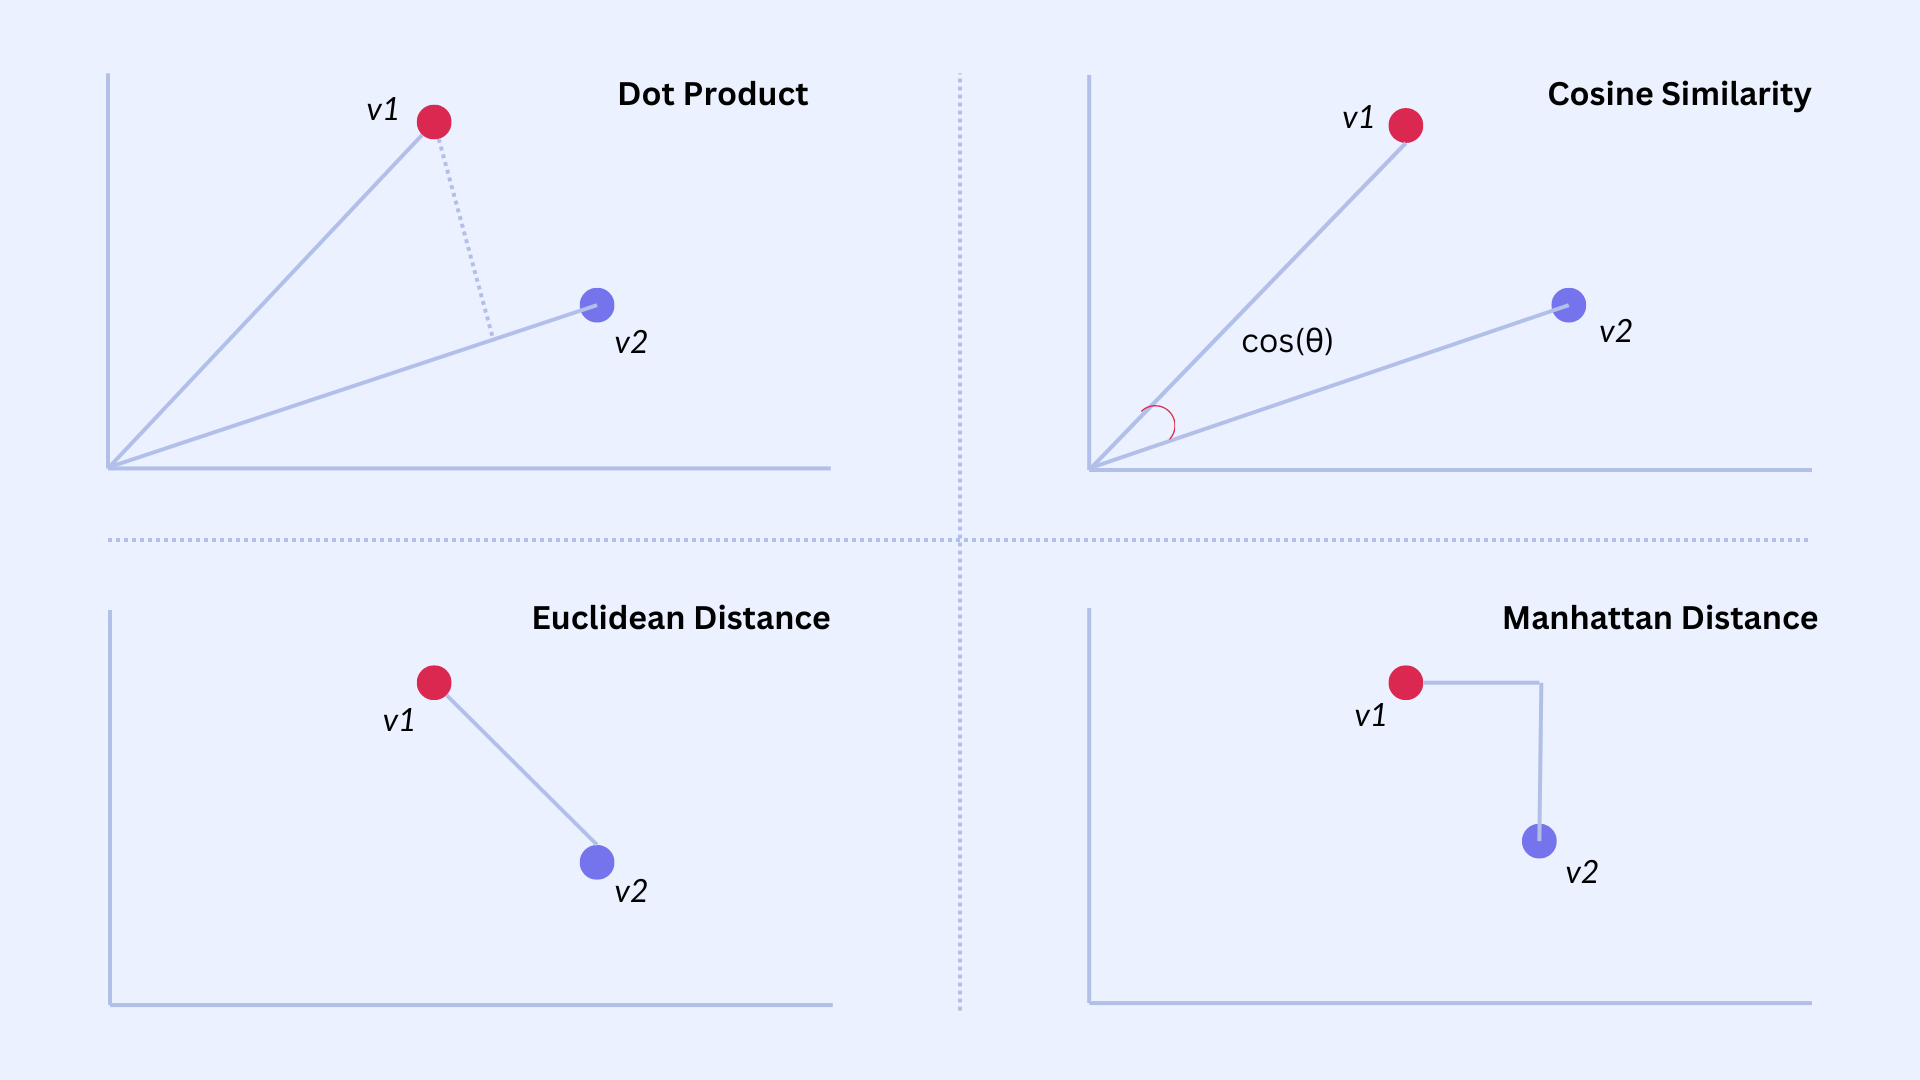
\includegraphics[width=0.75\linewidth]{Images/Kienthucnentang/vector-similarity.png}
    \caption[Vector Similarity trong semantic space với các vector embedding có ngữ nghĩa tương tự được phân bố gần nhau hơn trong không gian nhiều chiều]{Vector Similarity trong semantic space với các vector embedding có ngữ nghĩa tương tự được phân bố gần nhau hơn trong không gian nhiều chiều \cite{qdrant2024vectorsimilarity}}
    \label{fig:vector-similarity}
\end{figure}

\Cref{fig:vector-similarity}, vector similarity cho phép hệ thống xác định mức độ liên quan ngữ nghĩa giữa dữ liệu thông qua khoảng cách trong embedding space thay vì chỉ dựa trên keyword matching.
\subsubsection{Approximate Nearest Neighbor Search (ANN)}
Trong các hệ thống semantic search hiện đại, dữ liệu thường được biểu diễn dưới dạng vector embedding trong không gian nhiều chiều. Khi số lượng vector tăng lớn, việc tìm kiếm exact nearest neighbor trở nên tốn kém về thời gian và chi phí tính toán.

ANN là kỹ thuật tìm kiếm vector gần đúng nhằm tăng tốc quá trình retrieval trong không gian vector nhiều chiều \parencite{arya1998optimal}. Thay vì tìm vector gần nhất tuyệt đối, ANN chấp nhận kết quả gần đúng để đổi lấy thời gian truy xuất nhanh hơn.

ANN được sử dụng rộng rãi trong:
\begin{itemize}
    \item Semantic Search
    \item Vector Database
    \item Recommendation System
    \item Multimodal Retrieval
    \item Retrieval-Augmented Generation (RAG)
\end{itemize}

Các thuật toán ANN hiện đại như HNSW cho phép giảm đáng kể thời gian retrieval nhưng vẫn duy trì chất lượng tìm kiếm ở mức phù hợp cho semantic retrieval.

\begin{figure}[H]
    \centering
    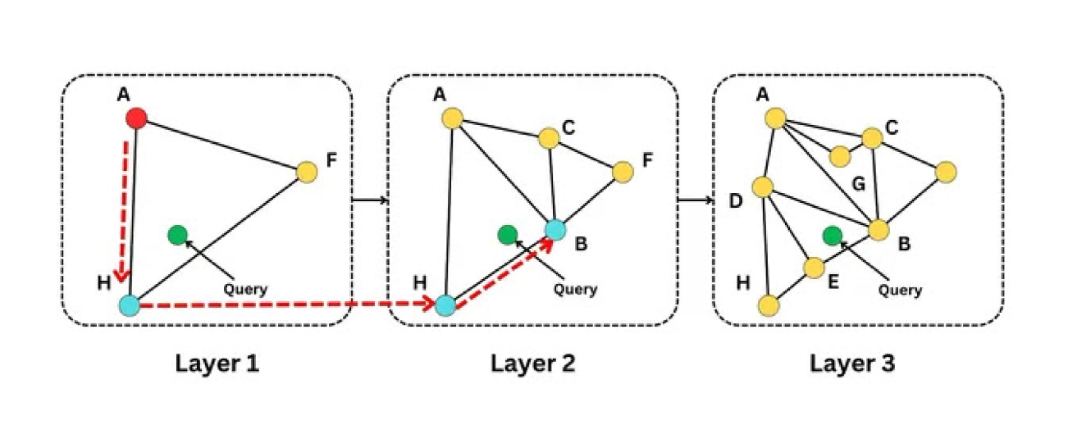
\includegraphics[width=1\linewidth]{Images/Kienthucnentang/ann-search-overview.png}
    \caption[Cơ chế Approximate Nearest Neighbor Search với quá trình truy xuất vector gần đúng nhằm tăng tốc tìm kiếm trong không gian vector nhiều chiều]{Cơ chế Approximate Nearest Neighbor Search với quá trình truy xuất vector gần đúng nhằm tăng tốc tìm kiếm trong không gian vector nhiều chiều \cite{analyticsvidhya2024ann}}
    \label{fig:ann-search-overview}
\end{figure}

\Cref{fig:ann-search-overview}, ANN search giúp hệ thống thực hiện vector retrieval hiệu quả trên tập dữ liệu lớn bằng cách giảm chi phí tìm kiếm trong không gian vector nhiều chiều.
\subsubsection{Hierarchical Navigable Small World (HNSW)}

HNSW là thuật toán Approximate Nearest Neighbor phổ biến trong các hệ thống semantic retrieval và vector database hiện đại \parencite{malkov2018efficient}.

HNSW xây dựng cấu trúc đồ thị nhiều tầng, trong đó mỗi node đại diện cho một vector embedding và các vector tương tự được kết nối với nhau. Quá trình tìm kiếm bắt đầu từ các tầng trên để nhanh chóng thu hẹp không gian tìm kiếm, sau đó tiếp tục refinement ở các tầng thấp hơn nhằm tìm nearest neighbor phù hợp.

Nhờ cơ chế tìm kiếm heuristic trên đồ thị phân tầng, HNSW giúp giảm đáng kể số lượng vector cần so sánh nhưng vẫn duy trì chất lượng retrieval cao.

Một số ưu điểm của HNSW gồm:
\begin{itemize}
    \item Tốc độ retrieval nhanh.
    \item Recall cao trong ANN search.
    \item Khả năng mở rộng tốt trên dữ liệu lớn.
\end{itemize}

Hiện nay, HNSW được sử dụng rộng rãi trong các vector database như Qdrant, Weaviate và Elasticsearch Vector Search.

\begin{figure}[H]
    \centering
    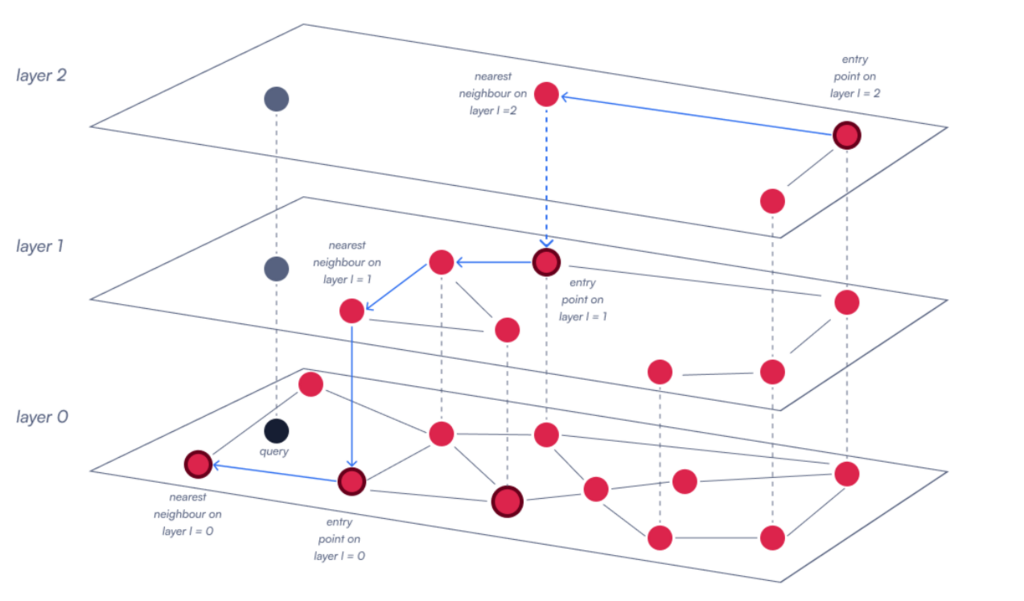
\includegraphics[width=0.75\linewidth]{Images/Kienthucnentang/hnsw-overview.png}
    \caption[Cấu trúc đồ thị phân tầng của thuật toán Hierarchical Navigable Small World (HNSW) trong Approximate Nearest Neighbor Search]{Cấu trúc đồ thị phân tầng của thuật toán Hierarchical Navigable Small World (HNSW) trong Approximate Nearest Neighbor Search \cite{qdrant2024hnsw}}
    \label{fig:hnsw-overview}
\end{figure}

\Cref{fig:hnsw-overview}, HNSW sử dụng cấu trúc đồ thị phân tầng để tăng tốc quá trình vector retrieval trong semantic search.

\subsection{Query Understanding và Query Processing}

\subsubsection{Query Understanding}

Query Understanding là quá trình phân tích truy vấn nhằm xác định ý định tìm kiếm và ngữ nghĩa của người dùng \parencite{guo2020deep}. Trong các hệ thống AI Search hiện đại, query understanding giúp hệ thống hiểu semantic meaning thay vì chỉ dựa trên keyword matching.

Trong thực tế, người dùng có thể sử dụng nhiều cách diễn đạt khác nhau cho cùng một nhu cầu tìm kiếm. Ví dụ, ``giày chạy bộ'', ``running shoes'' và ``sports sneakers'' có thể mang ý nghĩa tương tự dù khác từ vựng.

Mục tiêu của query understanding là chuyển đổi truy vấn thành semantic representation nhằm hỗ trợ retrieval và ranking hiệu quả hơn.

Một số thành phần chính của query understanding gồm:
\begin{itemize}
    \item Intent Understanding
    \item Semantic Representation
    \item Context Understanding
    \item Entity Recognition
\end{itemize}

Query understanding hiện được ứng dụng rộng rãi trong semantic search, recommendation system và conversational AI nhằm cải thiện chất lượng retrieval và độ liên quan của kết quả tìm kiếm.

\subsubsection{Query Expansion}

Query Expansion là kỹ thuật mở rộng truy vấn nhằm bổ sung các từ khóa hoặc biểu diễn ngữ nghĩa liên quan để cải thiện khả năng retrieval \parencite{carpineto2012survey}. Phương pháp này giúp hệ thống truy xuất dữ liệu hiệu quả hơn khi truy vấn ban đầu quá ngắn hoặc thiếu ngữ cảnh.

Một số hướng tiếp cận phổ biến gồm:

\begin{itemize}
    \item Synonym Expansion
    
    \item Semantic Expansion
    
    \item Knowledge-based Expansion
    
    \item Embedding-based Expansion
\end{itemize}

Ví dụ, truy vấn ``running shoes'' có thể được mở rộng thành ``sports sneakers'' hoặc ``giày chạy bộ'' nhằm tăng khả năng truy xuất các sản phẩm liên quan.

Query expansion hiện được sử dụng rộng rãi trong semantic search, recommendation system và conversational AI để cải thiện recall và semantic retrieval.

\subsubsection{Query Rewrite}

Query Rewrite là kỹ thuật chuyển đổi hoặc chuẩn hóa truy vấn nhằm tạo ra biểu diễn phù hợp hơn cho quá trình retrieval \parencite{ren2010query}. Phương pháp này giúp hệ thống xử lý các truy vấn viết tắt, sai chính tả hoặc diễn đạt không chuẩn nhưng vẫn giữ nguyên ý định tìm kiếm của người dùng.

Một số dạng query rewrite phổ biến gồm:

\begin{itemize}
    \item Spelling Correction
    
    \item Query Normalization
    
    \item Paraphrase Rewrite
    
    \item Context-aware Rewrite
\end{itemize}

Ví dụ, truy vấn ``nik running shose'' có thể được chuẩn hóa thành ``nike running shoes'' để cải thiện chất lượng retrieval.

Query rewrite hiện được sử dụng rộng rãi trong semantic search và conversational AI nhằm nâng cao khả năng hiểu truy vấn và semantic retrieval.

\subsubsection{Metadata Filtering}

Metadata Filtering là kỹ thuật lọc dữ liệu dựa trên các thuộc tính mô tả đi kèm với đối tượng trong quá trình retrieval. Phương pháp này cho phép hệ thống kết hợp tìm kiếm ngữ nghĩa với các điều kiện cụ thể như danh mục, thương hiệu, khoảng giá hoặc trạng thái còn hàng, từ đó giúp kết quả trả về phù hợp hơn với nhu cầu của người dùng.

Trong hệ thống E-commerce, metadata thường bao gồm các thông tin như danh mục sản phẩm, khoảng giá, thương hiệu, màu sắc, kích thước, trạng thái còn hàng hoặc thời gian tạo dữ liệu. Đây là các thuộc tính không nhất thiết phản ánh trực tiếp nội dung ngữ nghĩa của sản phẩm, nhưng lại đóng vai trò quan trọng trong việc giới hạn phạm vi tìm kiếm.

Metadata filtering có thể được triển khai dưới nhiều dạng khác nhau, chẳng hạn như lọc theo khoảng giá, lọc theo danh mục, lọc theo thuộc tính sản phẩm hoặc lọc theo điều kiện đúng sai. Ví dụ, với truy vấn ``nike running shoes under 2 million'', hệ thống có thể sử dụng semantic search để hiểu ý định tìm kiếm giày chạy bộ, đồng thời áp dụng metadata filtering để giới hạn kết quả theo thương hiệu Nike và mức giá dưới 2 triệu.

Trong các hệ thống AI Search, metadata filtering giúp kết quả truy xuất trở nên chính xác và phù hợp hơn với nhu cầu thực tế của người dùng. Thay vì chỉ trả về các sản phẩm có vector embedding gần với truy vấn, hệ thống còn có thể loại bỏ những sản phẩm không thỏa mãn điều kiện cụ thể như sai danh mục, vượt quá ngân sách hoặc không còn hàng.

Metadata filtering hiện được sử dụng rộng rãi trong vector database, recommendation system và semantic search nhằm hỗ trợ retrieval có điều kiện trên tập dữ liệu lớn.
% \subsubsection{Fusion Strategy}

% Fusion Strategy là kỹ thuật kết hợp nhiều nguồn thông tin hoặc nhiều tín hiệu retrieval nhằm cải thiện chất lượng kết quả tìm kiếm \parencite{vogt1999fusion}. Trong các hệ thống AI Search hiện đại, dữ liệu retrieval thường được sinh ra từ nhiều phương pháp khác nhau như keyword search, vector search hoặc metadata filtering.

% Mục tiêu của fusion strategy là tổng hợp các tín hiệu retrieval để tạo ra ranking cuối cùng có mức độ relevance cao hơn so với việc sử dụng riêng lẻ từng phương pháp.

% Một số hướng tiếp cận fusion phổ biến bao gồm:

% \begin{itemize}
%     \item \textbf{Score Fusion}: Kết hợp điểm số từ nhiều retrieval model.
    
%     \item \textbf{Rank Fusion}: Kết hợp thứ hạng từ nhiều danh sách retrieval.
    
%     \item \textbf{Weighted Fusion}: Gán trọng số cho từng nguồn tín hiệu retrieval.
    
%     \item \textbf{Multimodal Fusion}: Kết hợp thông tin từ nhiều modality khác nhau.
% \end{itemize}

% Fusion strategy giúp hệ thống tận dụng ưu điểm của nhiều phương pháp retrieval khác nhau nhằm nâng cao chất lượng semantic search và recommendation \parencite{wu2022multimodal}.

\subsection{Large Language Model và AI Agent}

\subsubsection{Khái niệm Large Language Model}

Large Language Model (LLM) là các mô hình học sâu có quy mô lớn, được huấn luyện trên lượng dữ liệu văn bản rất lớn nhằm học cách biểu diễn, hiểu và sinh ngôn ngữ tự nhiên. Các mô hình này thường được xây dựng dựa trên kiến trúc Transformer, trong đó cơ chế self-attention cho phép mô hình xác định mối quan hệ giữa các token trong câu và xử lý ngữ cảnh của văn bản đầu vào \parencite{vaswani2017attention}.

Khác với các mô hình xử lý ngôn ngữ truyền thống thường được thiết kế cho từng tác vụ cụ thể, LLM có khả năng thực hiện nhiều tác vụ khác nhau thông qua cùng một mô hình nền tảng. Người dùng có thể cung cấp yêu cầu dưới dạng prompt, sau đó mô hình sẽ sinh phản hồi dựa trên ngữ cảnh và tri thức đã học được trong quá trình huấn luyện.

LLM có thể được ứng dụng trong nhiều tác vụ xử lý ngôn ngữ tự nhiên như:

\begin{itemize}
    \item Sinh và xử lý văn bản: sinh văn bản tự động, tóm tắt văn bản, dịch máy.
    \item Hiểu và khai thác thông tin: trả lời câu hỏi, phân loại văn bản, trích xuất thông tin.
    \item Hỗ trợ tương tác thông minh: suy luận ngôn ngữ, chatbot và AI assistant.
\end{itemize}

Một số thành phần quan trọng trong LLM bao gồm tokenization, token embedding, positional encoding, self-attention, Transformer layer và language modeling head. Trong đó, tokenization giúp chia văn bản thành các đơn vị nhỏ hơn, embedding chuyển các token thành vector số, còn self-attention giúp mô hình nắm bắt quan hệ ngữ cảnh giữa các từ hoặc cụm từ trong chuỗi đầu vào.

Trong các hệ thống AI Search và AI Shopping Assistant, LLM có thể được sử dụng để hiểu ý định tìm kiếm của người dùng, diễn giải truy vấn tự nhiên, tạo câu trả lời hội thoại, hỗ trợ gợi ý sản phẩm và kết hợp với Retrieval-Augmented Generation (RAG) để sinh phản hồi dựa trên dữ liệu được truy xuất từ hệ thống.

\subsubsection{Prompt Engineering}
Prompt Engineering là kỹ thuật xây dựng và điều chỉnh prompt để định hướng Large Language Model tạo ra phản hồi phù hợp với mục tiêu của người dùng. Prompt có thể được xem là phần đầu vào mà người dùng hoặc hệ thống cung cấp cho mô hình, bao gồm yêu cầu nhiệm vụ, ngữ cảnh, ràng buộc xử lý và định dạng đầu ra mong muốn.

Chất lượng prompt có ảnh hưởng trực tiếp đến chất lượng phản hồi của LLM. Một prompt rõ ràng, đầy đủ ngữ cảnh và có cấu trúc tốt sẽ giúp mô hình hiểu đúng yêu cầu, giảm khả năng sinh kết quả sai lệch và tăng tính nhất quán của đầu ra. Ngược lại, prompt mơ hồ hoặc thiếu thông tin có thể khiến mô hình trả lời không đúng trọng tâm hoặc tạo ra kết quả không phù hợp với mục tiêu của hệ thống.

Một prompt hiệu quả thường bao gồm các thành phần chính sau:

\begin{itemize}
    \item \textbf{Nội dung hướng dẫn}: bao gồm instruction, context và constraint, giúp mô hình hiểu nhiệm vụ, dữ liệu liên quan và các giới hạn cần tuân theo.
    \item \textbf{Định dạng và ví dụ}: bao gồm output format và example, giúp mô hình tạo đầu ra đúng cấu trúc và phù hợp với mong muốn của người dùng.
\end{itemize}

Một số dạng prompting phổ biến gồm:

\begin{itemize}
    \item \textbf{Zero-shot và Few-shot Prompting}: zero-shot không cung cấp ví dụ mẫu, còn few-shot cung cấp một vài ví dụ đầu vào và đầu ra để mô hình phản hồi theo mẫu.
    \item \textbf{Instruction và Chain-of-Thought Prompting}: instruction prompting sử dụng hướng dẫn rõ ràng, còn chain-of-thought prompting khuyến khích mô hình trình bày các bước suy luận trước khi đưa ra kết quả cuối cùng.
\end{itemize}

Trong các hệ thống E-commerce, Prompt Engineering có thể được sử dụng để điều khiển cách AI assistant trả lời người dùng, diễn giải truy vấn tìm kiếm, trích xuất thuộc tính sản phẩm, tạo mô tả sản phẩm hoặc sinh câu trả lời dựa trên kết quả truy xuất. Ví dụ, với truy vấn ``tìm laptop cho sinh viên học lập trình giá dưới 20 triệu'', prompt có thể hướng dẫn LLM xác định các tiêu chí như mục đích sử dụng, khoảng giá, hiệu năng, dung lượng RAM và mức độ phù hợp của từng sản phẩm.

Prompt Engineering hiện được sử dụng rộng rãi trong chatbot, AI assistant, hệ thống hỏi đáp, hệ thống tìm kiếm thông minh và các ứng dụng reasoning dựa trên LLM.

\subsubsection{Function Calling}

Function Calling là cơ chế cho phép Large Language Model kết nối và sử dụng các hàm, API hoặc công cụ bên ngoài để mở rộng khả năng xử lý. Thay vì chỉ sinh văn bản từ tri thức đã học, mô hình có thể xác định khi nào cần gọi công cụ, truyền tham số phù hợp và sử dụng kết quả trả về để tạo phản hồi cuối cùng cho người dùng.

Cơ chế này đặc biệt hữu ích trong các bài toán yêu cầu dữ liệu động hoặc thao tác với hệ thống bên ngoài. Ví dụ, LLM có thể gọi API để tra cứu thông tin sản phẩm, kiểm tra tồn kho, lấy giá hiện tại, truy vấn cơ sở dữ liệu, tạo đơn hàng hoặc lọc danh sách sản phẩm theo điều kiện cụ thể.

Một hệ thống Function Calling thường bao gồm các thành phần chính sau:

\begin{itemize}
    \item \textbf{Function Schema}: Mô tả tên hàm, mục đích sử dụng, danh sách tham số và kiểu dữ liệu đầu vào.
    \item \textbf{Tool Selection}: Quá trình mô hình xác định công cụ hoặc hàm phù hợp với yêu cầu của người dùng.
    \item \textbf{Tool Invocation}: Quá trình gọi hàm với các tham số được mô hình suy luận từ prompt.
    \item \textbf{Structured Output}: Kết quả được trả về dưới dạng có cấu trúc, giúp hệ thống dễ xử lý và kiểm tra.
    \item \textbf{Result Integration}: Kết hợp kết quả từ công cụ bên ngoài vào phản hồi cuối cùng của LLM.
\end{itemize}

Trong AI Shopping Assistant, Function Calling có thể được sử dụng để kết nối LLM với các dịch vụ nội bộ của hệ thống E-commerce. Khi người dùng đưa ra yêu cầu như ``tìm điện thoại dưới 10 triệu có pin tốt'', LLM có thể phân tích yêu cầu, gọi hàm tìm kiếm sản phẩm với các tham số như danh mục, khoảng giá và tiêu chí pin, sau đó tổng hợp kết quả để đưa ra gợi ý phù hợp.

Function Calling giúp LLM trở nên đáng tin cậy hơn trong các tác vụ cần dữ liệu chính xác và cập nhật, vì mô hình không cần tự suy đoán toàn bộ thông tin. Thay vào đó, mô hình có thể phối hợp với cơ sở dữ liệu, search engine, recommendation engine hoặc các API nghiệp vụ để tạo ra phản hồi có căn cứ hơn.

Nhờ khả năng kết nối giữa ngôn ngữ tự nhiên và các chức năng hệ thống, Function Calling hiện được sử dụng rộng rãi trong chatbot, AI assistant, AI agent và các hệ thống tự động hóa nhiều bước.

\subsubsection{Khái niệm AI Agent}

AI Agent là hệ thống trí tuệ nhân tạo có khả năng tiếp nhận thông tin, phân tích ngữ cảnh, thực hiện reasoning và đưa ra hành động nhằm đạt được một mục tiêu cụ thể \parencite{wooldridge2009introduction}. Khác với chatbot truyền thống chủ yếu phản hồi theo từng lượt hội thoại, AI Agent có thể tương tác với công cụ, dữ liệu hoặc môi trường bên ngoài để xử lý các tác vụ phức tạp hơn.

Một AI Agent thường bao gồm bốn thành phần chính: perception, reasoning, memory và action. Trong đó, perception giúp agent tiếp nhận thông tin đầu vào, reasoning hỗ trợ phân tích và lựa chọn hướng xử lý, memory lưu trữ ngữ cảnh hoặc lịch sử tương tác, còn action cho phép agent thực hiện hành động như gọi API, truy xuất dữ liệu hoặc tạo phản hồi cho người dùng.

Trong hệ thống AI Shopping Assistant, AI Agent có thể hỗ trợ người dùng tìm kiếm sản phẩm, lọc kết quả theo nhu cầu, so sánh sản phẩm và đưa ra gợi ý phù hợp. Nhờ khả năng kết hợp giữa hiểu ngôn ngữ tự nhiên và sử dụng công cụ bên ngoài, AI Agent được ứng dụng rộng rãi trong conversational AI, recommendation system và các hệ thống trợ lý thông minh.
\subsection{Retrieval-Augmented Generation (RAG)}
\subsubsection{Khái niệm RAG}

Retrieval-Augmented Generation (RAG) là kiến trúc kết hợp giữa khả năng truy xuất thông tin và khả năng sinh ngôn ngữ của Large Language Model nhằm hỗ trợ tạo ra phản hồi có độ chính xác và tính cập nhật cao hơn \parencite{lewis2020rag}.

Trong các mô hình ngôn ngữ truyền thống, tri thức chủ yếu được lưu trữ trong tham số của mô hình sau quá trình huấn luyện. Tuy nhiên, các mô hình này thường gặp hạn chế về khả năng cập nhật kiến thức mới hoặc truy xuất thông tin chuyên biệt theo từng miền dữ liệu. RAG được đề xuất nhằm giải quyết vấn đề này bằng cách cho phép hệ thống truy xuất thêm dữ liệu từ nguồn tri thức bên ngoài trước khi sinh phản hồi.

Về mặt nguyên lý, RAG hoạt động bằng cách kết hợp truy vấn của người dùng với các tài liệu liên quan được truy xuất từ knowledge base. Các tài liệu này đóng vai trò context bổ sung cho mô hình ngôn ngữ trong quá trình sinh câu trả lời.

RAG hiện được sử dụng rộng rãi trong nhiều hệ thống AI hiện đại như semantic search, chatbot, AI assistant và question answering system nhờ khả năng:
\begin{itemize}
    \item Giảm hiện tượng hallucination
    
    \item Tăng khả năng grounding vào dữ liệu thực tế
    
    \item Hỗ trợ truy xuất tri thức quy mô lớn
    
    \item Cải thiện độ chính xác của phản hồi
\end{itemize}

\subsubsection{Kiến trúc RAG}

Kiến trúc RAG thường bao gồm hai thành phần chính là retrieval module và generation module.

\begin{itemize}
    \item \textbf{Retrieval Module}: Thành phần chịu trách nhiệm truy xuất các tài liệu liên quan từ kho tri thức.
    
    \item \textbf{Generation Module}: Thành phần sử dụng thông tin truy xuất được để sinh phản hồi ngôn ngữ tự nhiên.
\end{itemize}

Trong quy trình hoạt động của RAG, truy vấn đầu vào trước tiên được chuyển đổi thành semantic representation thông qua embedding model. Sau đó, hệ thống thực hiện retrieval trên vector database hoặc knowledge base để tìm các tài liệu có mức độ liên quan cao. Các tài liệu này sẽ được kết hợp với truy vấn ban đầu và đưa vào mô hình ngôn ngữ để sinh câu trả lời cuối cùng.
\begin{figure}[H]
    \centering
    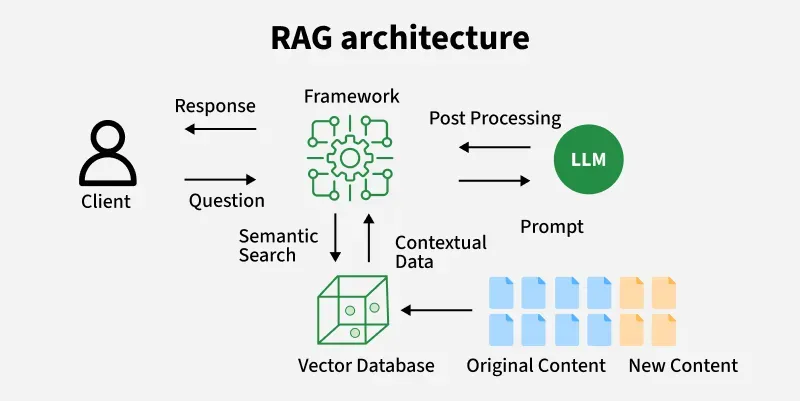
\includegraphics[width=0.75\textwidth]{Images/Kienthucnentang/RAG-architecture.png}
    \caption[Minh họa kiến trúc Retrieval-Augmented Generation (RAG)]{Minh họa kiến trúc Retrieval-Augmented Generation (RAG) \parencite{geeksforgeeks2026ragarchitecture}}
    \label{fig:rag-architecture}
\end{figure}
Kiến trúc RAG giúp hệ thống kết hợp đồng thời:
\begin{itemize}
    \item Khả năng semantic retrieval
    
    \item Khả năng reasoning của LLM
    
    \item Khả năng sinh ngôn ngữ tự nhiên
\end{itemize}

Nhờ đó, RAG có thể hỗ trợ xử lý hiệu quả các bài toán yêu cầu truy xuất tri thức động hoặc dữ liệu chuyên biệt theo từng miền ứng dụng.

\subsubsection{Retriever và Generator}
Trong kiến trúc RAG, retriever và generator là hai thành phần cốt lõi ảnh hưởng trực tiếp đến chất lượng phản hồi của hệ thống. Retriever chịu trách nhiệm tìm kiếm và truy xuất các tài liệu liên quan, trong khi generator sử dụng thông tin được truy xuất để tạo ra câu trả lời cuối cùng.

Retriever là thành phần thực hiện truy xuất dữ liệu liên quan từ knowledge base hoặc vector database dựa trên truy vấn đầu vào. Trong các hệ thống semantic retrieval hiện đại, retriever thường sử dụng dense vector retrieval nhằm tìm kiếm dữ liệu dựa trên semantic similarity thay vì keyword matching truyền thống.

Một số nhiệm vụ chính của retriever bao gồm:
\begin{itemize}
    \item Biểu diễn truy vấn dưới dạng vector embedding
    
    \item Tìm kiếm các tài liệu liên quan
    
    \item Tối ưu recall trong quá trình retrieval
\end{itemize}

Generator là thành phần chịu trách nhiệm sinh phản hồi cuối cùng dựa trên truy vấn và các tài liệu được retriever cung cấp. Generator thường là Large Language Model với khả năng tổng hợp thông tin và sinh ngôn ngữ tự nhiên.

Generator có vai trò:
\begin{itemize}
    \item Tổng hợp thông tin từ nhiều nguồn
    
    \item Thực hiện reasoning trên context truy xuất
    
    \item Sinh phản hồi tự nhiên và mạch lạc
\end{itemize}

Sự kết hợp giữa retriever và generator giúp hệ thống vừa có khả năng truy xuất thông tin chính xác vừa đảm bảo chất lượng phản hồi ngôn ngữ tự nhiên.

\subsubsection{Conversation Memory}

Conversation Memory là cơ chế giúp hệ thống conversational AI lưu trữ và duy trì ngữ cảnh trong quá trình hội thoại. Nhờ cơ chế này, hệ thống có thể ghi nhớ nội dung đã trao đổi trước đó và tạo ra phản hồi nhất quán hơn trong các cuộc hội thoại nhiều lượt.

Trong thực tế, truy vấn hiện tại của người dùng thường phụ thuộc vào các lượt hội thoại trước. Ví dụ, người dùng có thể hỏi ``sản phẩm này có rẻ hơn không'' sau khi vừa xem một danh sách sản phẩm. Nếu không có memory, hệ thống sẽ khó xác định người dùng đang nhắc đến sản phẩm nào.

Conversation Memory có thể được triển khai dưới nhiều dạng như lịch sử hội thoại, bản tóm tắt ngữ cảnh, context embedding hoặc bộ nhớ ngoài lưu trong cơ sở dữ liệu. Trong các hệ thống RAG, memory thường được kết hợp với retrieval mechanism để truy xuất thông tin theo ngữ cảnh, từ đó cải thiện khả năng reasoning và chất lượng phản hồi.

\subsubsection{Agentic RAG}

Agentic RAG là hướng mở rộng của Retrieval-Augmented Generation, trong đó mô hình ngôn ngữ không chỉ thực hiện truy xuất và sinh phản hồi theo một pipeline cố định, mà còn hoạt động như một AI agent có khả năng reasoning, lựa chọn hành động và sử dụng công cụ trong quá trình xử lý truy vấn \parencite{yao2023react}.

Khác với RAG truyền thống có pipeline tương đối cố định, Agentic RAG cho phép hệ thống linh hoạt quyết định khi nào cần truy xuất thông tin, khi nào cần suy luận, khi nào cần gọi external tools và khi nào sinh phản hồi cuối cùng. Quá trình xử lý có thể diễn ra theo nhiều vòng lặp giữa retrieve, reason và generate để từng bước hoàn thiện câu trả lời.

Một số đặc điểm nổi bật của Agentic RAG gồm multi-step reasoning, dynamic retrieval, tool usage integration và adaptive decision making. Nhờ các đặc điểm này, hệ thống có thể xử lý tốt hơn các truy vấn phức tạp, truy vấn nhiều điều kiện hoặc các tác vụ yêu cầu reasoning đa bước.

Trong hệ thống AI Shopping Assistant, Agentic RAG có thể hỗ trợ các yêu cầu như tìm kiếm sản phẩm theo nhiều tiêu chí, so sánh sản phẩm, lọc theo ngân sách, kiểm tra tồn kho hoặc giải thích lý do đề xuất. Vì vậy, Agentic RAG là hướng tiếp cận quan trọng trong các hệ thống AI assistant hiện đại nhờ khả năng kết hợp retrieval, reasoning và hành động trong cùng một quy trình xử lý.
\subsection*{Kết chương}

Chương này đã trình bày các kiến thức nền tảng phục vụ cho việc xây dựng hệ thống tìm kiếm thông minh trong thương mại điện tử. Nội dung chương bao gồm bài toán tìm kiếm sản phẩm, hạn chế của keyword-based search, semantic search, multimodal search và vai trò của AI trong việc cải thiện chất lượng tìm kiếm.

Bên cạnh đó, chương đã giới thiệu các nền tảng quan trọng của hệ thống truy hồi thông tin như BM25, semantic retrieval, vector embedding, vector similarity, vector database, ANN và HNSW. Đây là các thành phần giúp hệ thống biểu diễn dữ liệu dưới dạng vector và truy xuất kết quả phù hợp trong không gian ngữ nghĩa.

Chương cũng trình bày các kỹ thuật xử lý truy vấn như query understanding, query expansion, query rewrite và metadata filtering nhằm nâng cao độ chính xác của kết quả retrieval. Ngoài ra, các nội dung về Computer Vision, Text-Image Retrieval và Object Detection làm rõ cách hệ thống khai thác dữ liệu hình ảnh trong tìm kiếm sản phẩm.

Cuối cùng, chương đã giới thiệu các khái niệm về Large Language Model, AI Agent và Retrieval-Augmented Generation, bao gồm prompt engineering, function calling, conversation memory và Agentic RAG. Những kiến thức này là cơ sở để thiết kế hệ thống AI Shopping Assistant có khả năng hiểu truy vấn, truy xuất dữ liệu, suy luận và sinh phản hồi tự nhiên trong các chương tiếp theo.